\section{Experiments}~\label{experiment}
Our experiments examine the proposed system through two complementary layers. In the system evaluation, an oracle user always provides correct answers to robot queries, and we measure task success, execution length, and query frequency as properties of the planning framework. We first analyze how the confidence threshold $\tau$ affects these measures. We then compare four feedback strategies: \textbf{All}, \textbf{No}, \textbf{Random}, and \textbf{Ours}. The user study examines how the resulting query styles shape user performance, workload, and situation awareness with actual participants.

\begin{figure}[t!]
    %\captionsetup{skip=0pt} % \hspace{0.3cm}
    \begin{center}
  
    \begin{subfigure}[b]{0.47\textwidth}
        \captionsetup{skip=0pt}
	    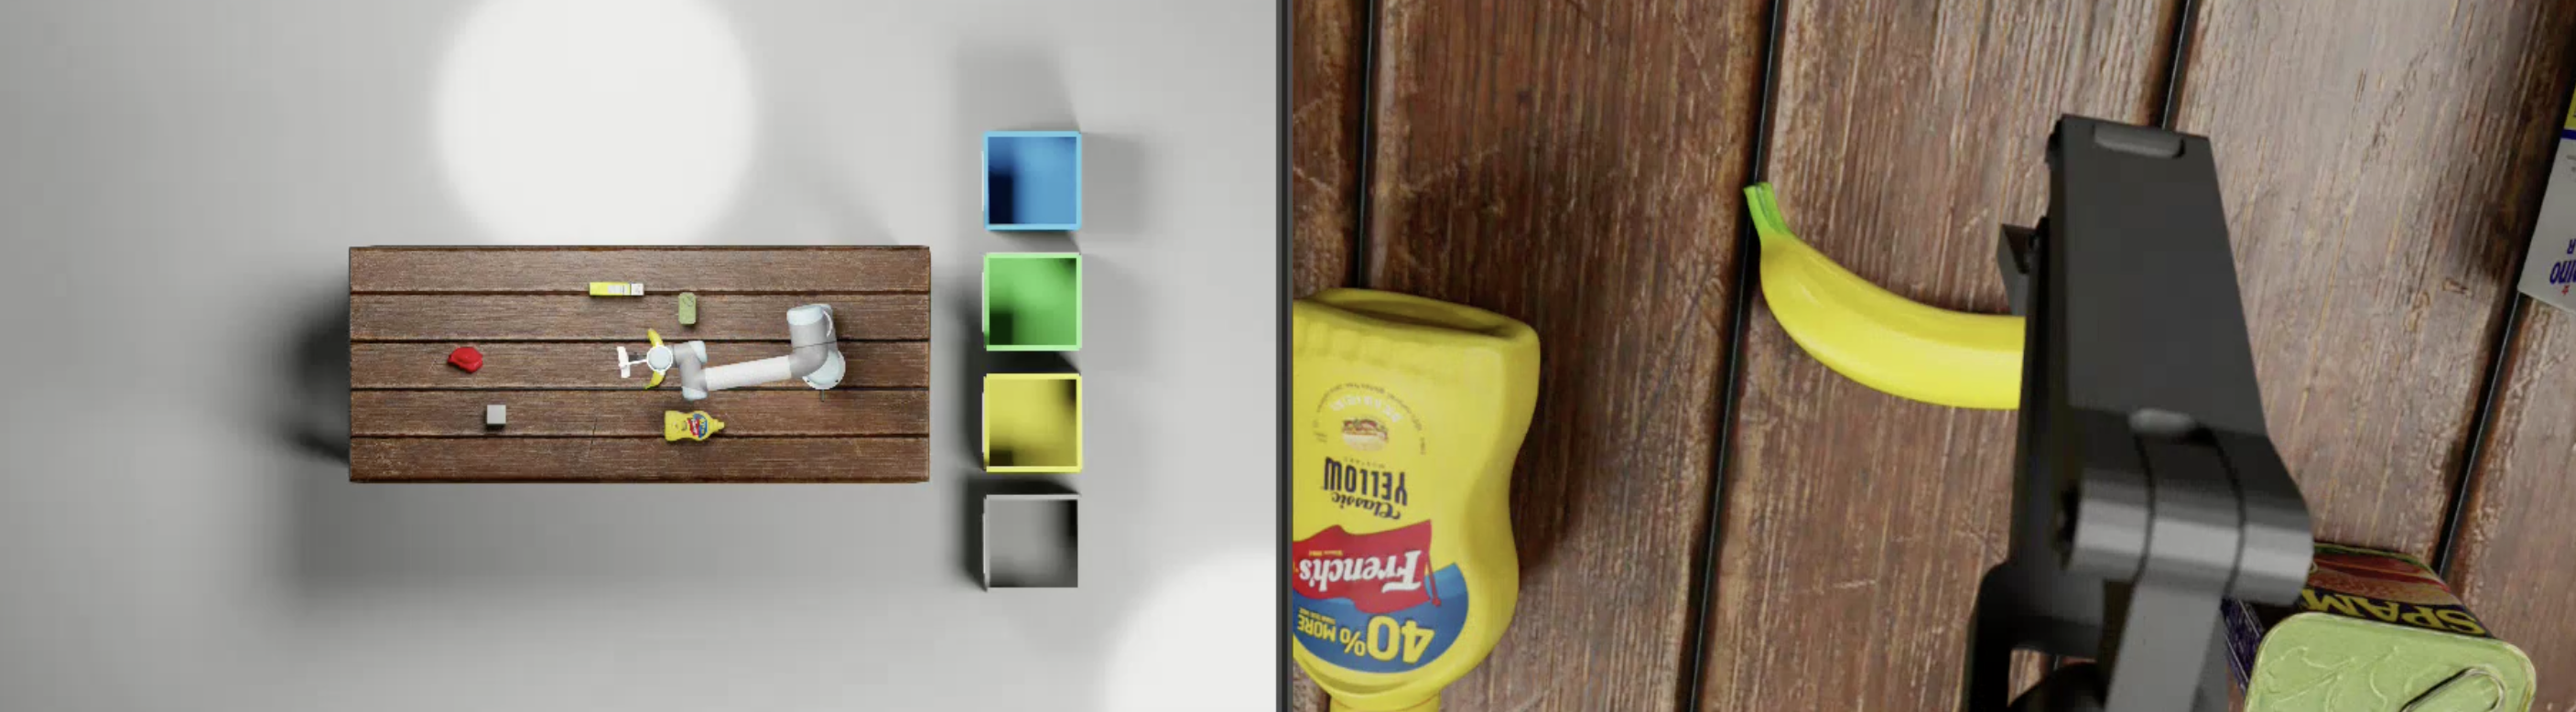
\includegraphics[width=\textwidth]{figures/fig_exp_setup1.png}
        \caption{Waste sorting domain overview. }
        \label{fig:dom1}
    \end{subfigure}
    \quad
    \begin{subfigure}[b]{0.47\textwidth}
        \captionsetup{skip=0pt}
	    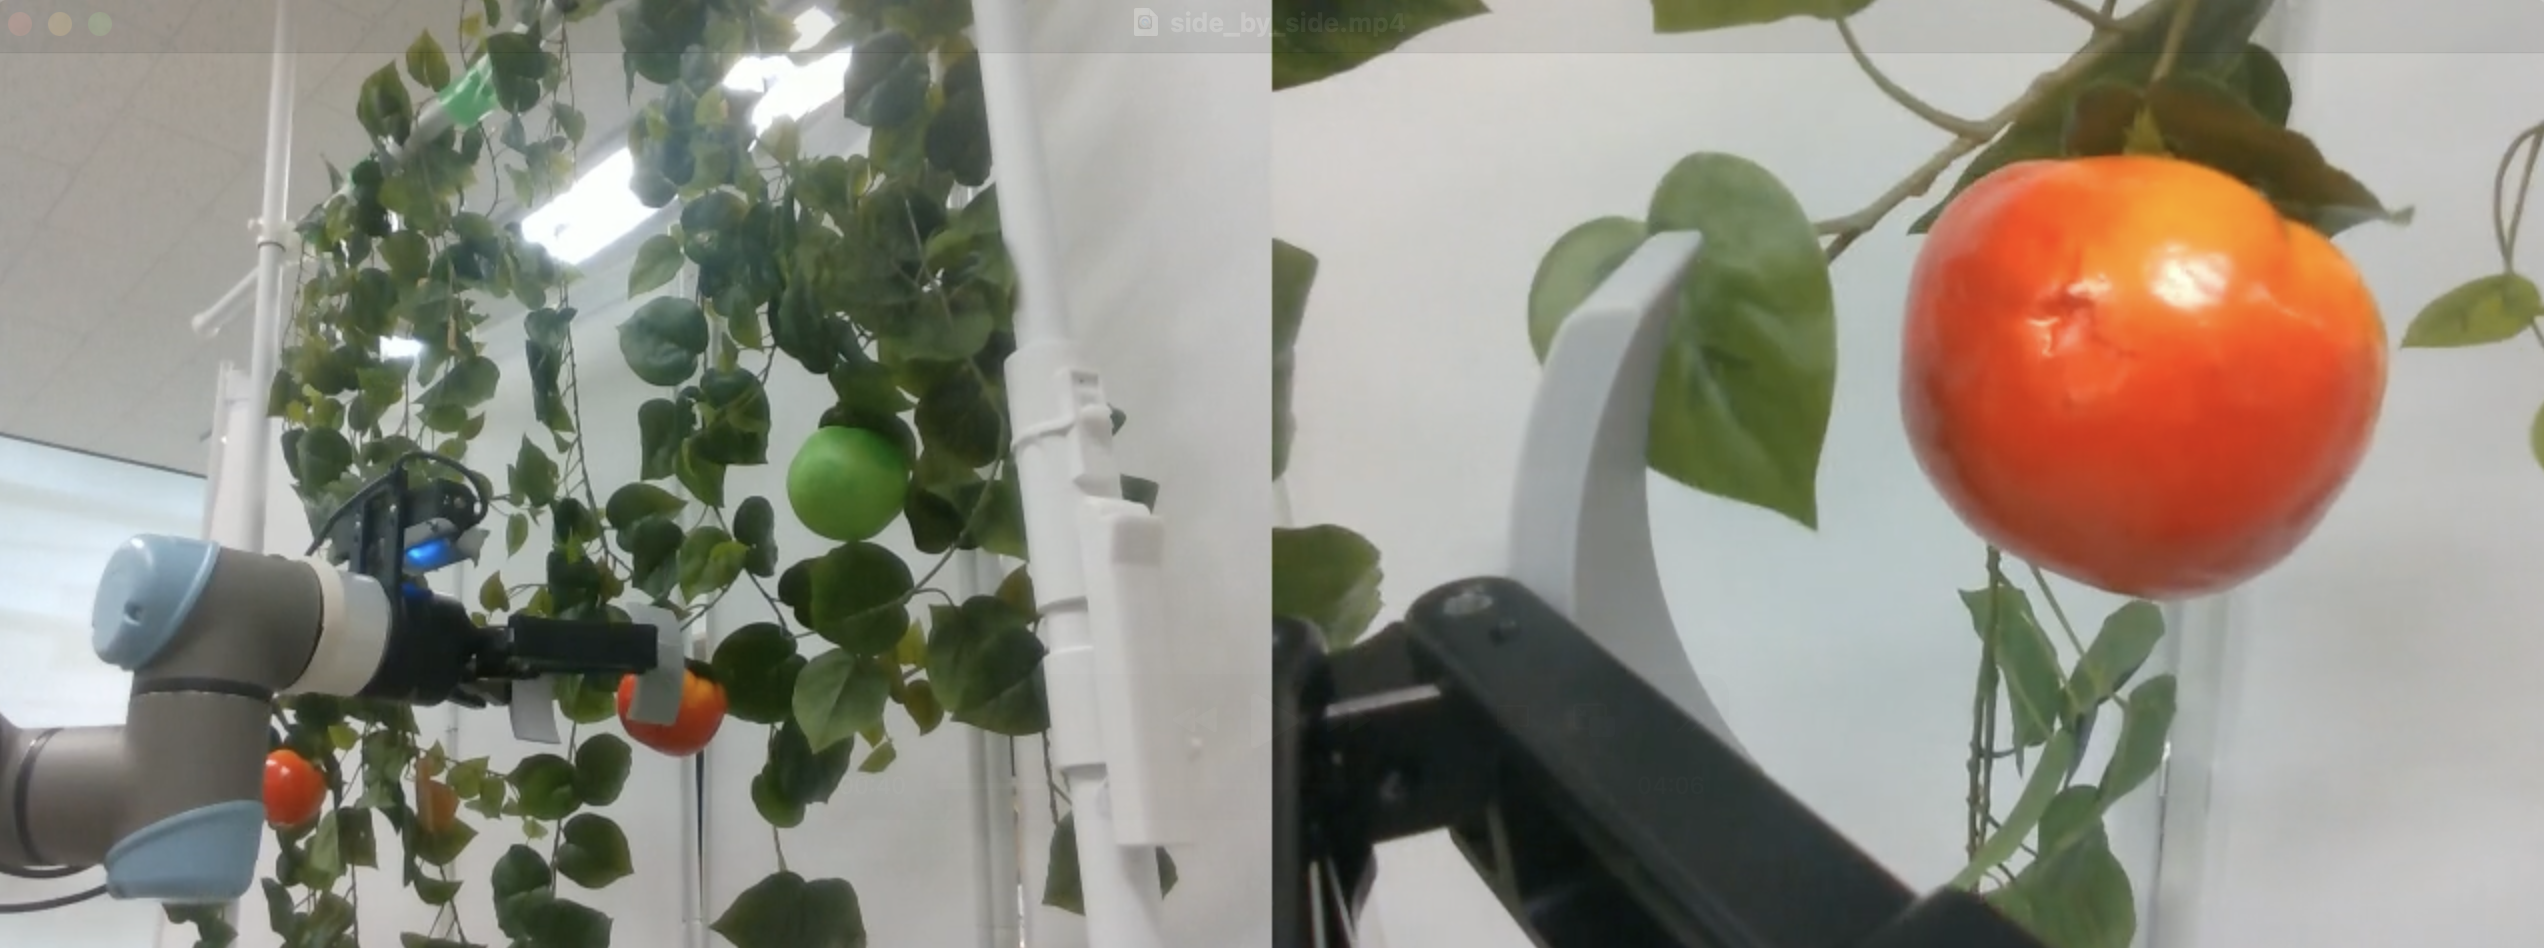
\includegraphics[width=\textwidth]{figures/fig_exp_setup2.png}
        \caption{Tomato harvesting domain overview}
        \label{fig:dom2}
    \end{subfigure}
    \caption{The illustration of the environments. (a) A UR5 robot sorts four types of waste into designated bins in Isaac Sim. (b) A mobile manipulator harvests ripe tomatoes and discards rotten ones in a real-world setting.}
  \label{fig:env_setting}
  
  \end{center}
\end{figure}


\subsection{Experimental Setup}~\label{exp:setup}
The experimental setup includes a simulated waste sorting domain and a real-world tomato harvesting domain. For waste sorting, NVIDIA Isaac Sim provides a tabletop environment with a fixed UR5 robotic arm for pick-and-place tasks. For tomato harvesting, a Summit mobile platform carries a UR5e robotic arm and operates in a lab environment. The mobile platform uses an RGB-D camera for visual perception and a LiDAR sensor for localization. Both domains use YOLOv12 for object detection~\cite{tian2025yolov12}.


\subsubsection{Waste sorting domain}~\label{exp:setup_waste}
As shown in Fig.~\ref{fig:dom1}, a fixed UR5 robot is positioned between the objects and the recycling bins and performs three actions: \texttt{detect}, \texttt{pick}, and \texttt{place}. We assume that all objects are reachable by the manipulator.

Each object belongs to one of four categories: \texttt{general}, \texttt{paper}, \texttt{can}, and \texttt{plastic}. The object categories are not known a priori and must be inferred through perception. Since objects may be partially occluded by others, a single observation may not reveal all categories, requiring repeated detection during execution. The \texttt{detect} action can observe multiple objects simultaneously, after which the robot places each object into the corresponding recycling bin.

The initial arrangement of objects is randomized in every episode. A task is considered successful when all objects are correctly sorted within the maximum step limit. A reward of $+5$ is assigned when a waste object is placed into the recycling bin corresponding to its category, and an additional reward of $+10$ is given when all objects are correctly sorted. All other actions receive zero reward.



\subsubsection{Tomato harvesting domain}~\label{exp:setup_tomato}
We consider a tomato harvesting scenario in which four tomatoes are attached to two stems, denoted as \texttt{stem\_1} and \texttt{stem\_2}, as shown in Fig.~\ref{fig:dom2}. The robot navigates between three locations: \texttt{dock\_station}, \texttt{stem\_1}, and \texttt{stem\_2}, and performs \texttt{detect}, \texttt{pick}, \texttt{scan}, \texttt{place}, and \texttt{discard} actions.

Each tomato can be in one of three states: \texttt{ripe}, \texttt{unripe}, or \texttt{rotten}. The tomato states are initially unknown and must be estimated through perception. During detection, ripe and rotten tomatoes are visually ambiguous and cannot always be reliably distinguished. To resolve this ambiguity, the robot performs a \texttt{scan} action after picking a tomato to verify its condition before harvesting or discarding it. Unripe tomatoes are left untouched.

The tomato locations are randomized across stems in every episode. A task is considered successful when all ripe tomatoes are harvested and all rotten tomatoes are discarded within the maximum step limit. A reward of $+5$ is assigned when a ripe tomato is correctly harvested or a rotten tomato is correctly discarded after scanning. An additional reward of $+10$ is given when all task-relevant tomatoes are processed correctly. All other actions receive zero reward.



\subsubsection{Implementation Details}~\label{exp:details}
In all experiments, the planner used a discount factor $\gamma=0.95$, UCB exploration constant $c=1.0$, maximum simulation depth $depth_{\max}=20$, and $\Timeout=100$ Monte Carlo simulations per planning step. Each episode was limited to $50$ steps. Each reported domain-threshold or domain-strategy result aggregates five scenario configurations with $200$ randomized episodes per scenario, yielding $1000$ episodes per domain-condition cell. Each episode was initialized with a pseudorandom seed that controls both Python \texttt{random} and NumPy sampling and is stored with the raw execution log.

The threshold-sweep experiment treats $\tau$ as the independent variable and is reported first in Sec.~\ref{exp:sys_results}. After observing that performance saturates for $\tau \geq 0.7$ while query frequency continues to increase, we use $\tau=0.8$ for the subsequent strategy-comparison experiment.
